    \chapter{Описание исследованных акваторий}
        \section{Географическое и физиономическое описание}
			\subsection{Белое море}

\subsubsection{Участок материковой литорали, расположенный в 800 м к югу от поселка Лувеньга.}

Данный разрез имеет вид прямоугольника, длина которого ограничена $10$~метрами, а ширина равна ширине литорали в максимальный сизигийный отлив (72 метра). 
На данном участке пробы брались равномерно на протяжении всей ширины литорали. 

Верхняя часть литорали на разрезе представляет гравийно-мелкокаменистую осыпь со значительным наклоном дна, нижняя граница которой расположена в 
$10$~метрах от штормовых выбросов.

Ниже на литорали располагается пологий пляж с илистым песком с заметными вкраплениями крупного песка. 
В данном биотопе отмечены отдельные выбросы пескожилов {\it Arenicola marina} и кое-где тонкий мат зеленых нитчаток. 
В дальнейшем эта зона будет называться <<верхний пляж>>. 
На расстоянии $19$~метров от штормовых выбросов верхний пляж ограничивает валунная гряда.

За валунной грядой следует валунная россыпь с плотными поселениями фукоидов. 
Постепенно россыпь разреживается и между валунами появляются окна илисто-песчаного грунта. 
Плотность пояса фукоидов также постепенно уменьшается, и к $37$~метру от штормовых выбросов фукоиды и валуны практически полностью исчезают. 
В дальнейшем этот биотоп будет называться <<пояс фукоидов>>.

Ниже располагается следующий хорошо различимый биотоп --- пояс взморника {\it Zostera marina}. 
Плотное, почти со стопроцентным проективным покрытием, поселение этих растений на илисто-песчаном грунте простирается до $59$~метра от штормовых выбросов. 
Помимо взморника, в данном биотопе отмечено большое количество нитчатых водорослей с прикрепленных на них молодью мидий {\it Mytilus edulis}.

От $59$ до $72$~метра расположен участок, осушающийся только в сизигийный отлив. 
Илисто-песчаный пляж данного биотопа служит местом обитания для поселений пескожила и большого количества мидиевых щеток. 
Данный биотоп будет именоваться <<нижний пляж>>. 


\subsubsection{Илистая губа острова Горелого.}
Ширина литорали на данном участке составляет $24$~метра. 
Так как верхняя литораль характеризуется каменистым грунтом, то пробы брались только в среднем и нижнем горизонте литорали.
Верхняя часть литорали представляет собой гравийную россыпь, выходящую на приморский луг. 
Ниже (в среднем горизонте) следует илисто-песчаный пляж с редкими некрупными камнями и отдельными выбросами пескожилов.  
На расстоянии $15$~метров от линии штормовых выбросов появляются редкие вкрапления фукоидов (на границе среднего и нижнего горизонтов литорали) и увеличивается количество мелких камней, но  все же этот участок можно характеризовать как илисто-песчаный пляж. 
Плотность поселения {\it Arenicola marina} заметно увеличивается по сравнению со средним горизонтом.
На уровне $17-21$ метров от штормовых выбросов располагается валунная гряда с плотными поселениями фукоидов (нижний горизонт литорали). 
В данной зоне пробы отбирались на участках, не закрытых талломами водорослей. 
В районе нуля глубин на данном участке также характерен илисто-песчаный грунт с плотным поселением {\it Arenicola marina}.


\subsubsection{Эстуарий реки Лувеньги.}
На данном участке ширина литорали составляет $500$~метров. 
На всем протяжении это практически горизонтальный илисто-песчаный пляж с плотным поселением пескожилов. 
Так как этот участок расположен в эстуарии реки, то он характеризуется пониженной соленостью. 
В данном районе пробы брались на расстоянии $350$~метров от линии штормовых выбросов на нижнем горизонте литорали.

\subsubsection{Западная Ряшкова Салма}
Литораль в точке исследования достигает ширины около $40$~метров.
Верхний горизонт литорали представлен каменистой россыпью, которая по мере продвижения в сторону моря становится более разреженной с пятнами песчаного грунта между камнями.
Средний горизонт литорали предсталвен илисто-песчаным пляжем с примесью гравия.
Нижний горизонт литорали представлен плотным поселением фукоидов на камнях.
На данном участке пробы отбирали в среднем горизонте литорали в пределах двух станций.


\subsubsection{Южная губа о.~Ряшкова}
В куту Южной губы литораль достигает ширины $250$~метров. 
На всем протяжении это пологий илисто-песчаный пляж с отдельными валунами и камнями, поросшимы фукоидами.
В губу спадает ручей, воды которого в отлив свободно разливаются по литорали и не образуют явного русла.
На данном участке пробы отбирали у нуля глубин западнее ручья в месте обитания хищных улиток \textit{Amauropsis islandica} (\cite{Aristov_Granovich_2011}).


\subsubsection{о.~Большой Ломнишный}
Литораль в точке исследования представляет собой пологую отмель шириной около $40$~метров.
Грунт представляет собой песок с примесью ила и крупных валунов.
Оформленный пояс фукоидов отсутствует, скопления фукоидов приурочены к отдельно лежащим валунам.
Пробы отбирали у нуля глубин в месте обитания хищных улиток \textit{Amauropsis islandica} (\cite{Aristov_Granovich_2011}).



            \subsection{Баренцево море}

            \subsubsection{Северное Нагорное}
Данный участок расположен в третьем колене Кольского залива, на южном его берегу в пределах одноименного района г.~Мурманск. 
Собственно литораль начинается за жилым массивом, в месте расположения опор моста через Кольский залив. 
Место сбора находилось в 600 м севернее моста. 
Ширина литорали на данном участке составляет $100$~м. 
Верхний горизонт литорали представлен небольшими валунами и россыпью гравия. 
Средний и нижний горизонты литорали представляют собой достаточно пологий илисто-песчаный склон с редкими валунами. 
Грунт достаточно сильно эвтрофицирован, очень вязкий. 
Между валунами встречаются поселения пескожила {\it Arenicola marina}.

            \subsubsection{Абрам-мыс}
Участок  в районе  Абрам-мыса  находится в третьем колене Кольского залива, максимально удаленном от моря.
Абрам-мыс --- район   города   Мурманск,  расположенный   на противоположной стороне залива от основного городского массива, напротив порта. 
Исследованный участок   литорали   находился   в   $1,5$~км   к   выходу   из   залива   от   причала,   куда   приходит пассажирский катер. 
Ширина   литорали   на   данном   участке   составляет   $45$~м.   
Верхний   горизонт   литорали представлен  каменисто-галичной  россыпью. 
В среднем  горизонте литорали на поверхности илисто-песчаного   грунта   располагаются   валуны,   покрытые   фукоидами   ({\it Fucus  vesiculosus}), которые   формируют   практически   сплошной   покров   с   отдельными   «окнами»   грунта (проективное  покрытие фукоидов $90~\%$).  
При приближении  к нижнему горизонту литорали количество   валунов   уменьшается,   и   проективное   покрытие   фукоидов   составляет   здесь   не более $10~\%$.

\subsubsection{Ретинское}
Ретинское находится на западном берегу Кольского залива, напротив г.~Североморск. 
В береговую линию вдается небольшая, овальной формы губа. 
Ширина литорали составляет около $60$~м. 
Дно каменистое, между камнями --- илисто-песчаный грунт, достаточно промытый. 
На верхнем горизонте литорали располагаются крупные валуны, покрытые фукусами и балянусами, чуть ниже находятся крупные камни полностью покрытые фукоидами.
Средний и нижний горизонты литорали представлены среднего размера камнями, примерно половина из которых покрыта фукоидами. 

\subsubsection{Пала-губа}
Пала-губа   представляет   собой   глубоко   вдающуюся   в   берег   губу   длинным   узким «горлом», за которым следует расширение, формирующее несколько губ второго порядка. 
В «горле» расположен остров Шалим, и, таким образом, губа соединяется с Кольским заливом узкими   проливами.   
В   основной   части   Пала-губы   расположено   несколько   более   мелких островков. 
Исследованный участок располагался в длинной узкой губе (бухта Дровяная), закрытой на выходе островом Зеленый.
В кут губы впадает крупный ручей, образующий на литорали во время отлива оформленное русло, положение которого за два года наблюдений не изменилось.
Ширина литорали на данном участке составляет  $130$~м. 
Верхний горизонт литорали представлен   каменисто-валунной   россыпью,   которая   на   границе   со   средним   горизонтом становится более разреженной, и покрыта зарослями фукоидов ({\it Fucus vesiculosus}). 
Средний и нижний   горизонты   представлены   двумя   илисто-песчаными   пляжами,   разделенными каменисто-валунной грядой на месте резкого локального увеличения угла уклона свала. 
На нижней литорали грунт более заилен, и на поверхности располагаются агрегации {\it Mylius edulis} («мидиевые щетки»).

\subsubsection{Печенга}
Печенга расположена на Западном Мурмане, в $150$~км от границы с Норвегией. 
Собственно поселок находится на берегу сильно вдающейся в полуостров губы Печенга. 
Сбор материала производился в средней части этой губы, на удалении $1,5$~км от кута губы. 
Литораль на этом участке достигает ширины $50$~м. 
Верхний горизонт литорали представлен среднего размера валунами. 
На среднем горизонте валуны расположены более редко, а между ними находится россыпь достаточно крупного гравия. 
Нижний горизонт литорали илисто-песчаный. 

\subsubsection{Губа Гаврилово}
Гаврилово – наиболее западная губа из исследованных нами участков на Восточном Мурмане. 
Эта   губа   с  достаточно   широким   входом,   свободно   открывающаяся  в  Баренцево море.   
Восточную   ее   часть   закрывает   от   прибоя   мыс,   формирующий   «горло», суженное относительно основной части. 
В восточной части кута губа формирует узкий отрог длиной   около $200$~м, по которому течет ручей, распадающийся в центральной части   губы  в  среднем   горизонте   литорали   на   два   рукава,   и   сливающиеся   ниже   обратно   в единое русло.
Ширина литорали  в  данной губе составляет  $500$~м  (без  учета отрога, дно которого полностью обнажается в отлив) Верхний горизонт литорали на данном участке представлен каменисто-галечной   россыпью.   
Средний   горизонт   литорали   представляет   собой   обширную илисто-песчаную   отмель   с   отдельными   камнями   и   валунами.  
В   основном   камни   и   валуны сконцентрированы   вдоль   русла   ручья.   
Нижний   горизонт   литорали   представлен   песчаным пляжем. 

\subsubsection{Губа Ярнышная}
Губа Ярнышная представляет собой одну из крупнейших губ Восточного Мурмана, ее длина составляет около $5$~км. 
Вход в губу свободно открыт в Баренцево море. 
Берега губы сильно изрезаны. 
В кут губы Ярнышной впадают два крупных ручья --- Ярнышный и Бобровый. 
По мере продвижения в кут губы, скальная и каменистая литораль переходит в каменисто-песчаную и илисто-песчаную. 
Исследованный участок расположен в юго-восточной части кута губы в районе впадения ручья Ярнышный.
На   участке   исследования   средний   горизонт   литорали   представлен   илисто-песчаным пляжем   с   отдельными   валунами,   поросшими   фукоидами   ({\it Fucus   vesiculosus}).   
В   среднем   и нижнем горизонте литорали вдоль русла ручья были остатки умершего плотного поселения  {\it Mytilus eduls} («мидиевая банка»), поэтому в период исследования в данном биотопе грунт был черный с запахом сероводорода.

\subsubsection{Губа Дальнезеленецкая}
Исследованный   участок   был   расположен   на   литоральной   отмели   Дальний   Пляж, поскольку именно он был в 1970х годах выбран как модель для описания литоральной фауны мягких   грунтов   на   Баренцевом   море.   
На   границе   верхней   литорали   расположен   валунно-галечный   пляж,  нижняя   часть которого заросла фукоидами ({\it Fucus vesiculosus}). 
Ниже по литорали в юго-восточной части пляжа   тянется   узкая   (около   $10-15$~м   шириной)   полоса   крупного   песка,   в   которой представители макробентоса практически отсутствуют.
Средний   горизонт   литорали --- это   обширный   илисто-песчаный   пляж,   в  пределах которого визуально выделяется три зоны: с преобладанием пескожилов  {\it Arenicola marina}, с преобладанием   мелких   полихет-трубкостроителей   (в   первую   очередь, {\it Fabricia   sabella})   и переходная   зона   между   этими   сообществами.   
Нижняя   литораль   представлена   каменисто-песчаным пляжем с зарослями бурых ({\it Fucus vesiculosus}, {\it Fucus serratus}) и красных ({\it Palmaria  palmata}) водорослей на камнях.

\subsubsection{Губа Шельпино}
Шельпино   представляет   собой   большую   губу   с   широким   горлом,   в   котором расположен   один   крупный   и   несколько   мелких   островов.   
В   юго-восточной   части   губа продолжается   длинным   (около   $400$~м)   узким   отрогом,   полностью   обнажающимся   в   отлив. 
Именно в этом отроге и происходил пробоотбор. 
По   литорали   отрога   протекает   небольшой   ручей,   не   формирующий   четкого   русла. 
Летом вдоль ручья развиваются массовые скопления зеленой водоросли рода  {\it Enteromorpha}. 
Верхняя и средняя литораль представляют собой песчаный пляж с отдельными камнями и валунами. 
В среднем горизонте на камнях появляются водоросли. 
Нижний горизонт литорали оккупирован плотным поселением мидий {\it Mytilus edulis} на грунте.

\subsubsection{Губа Порчниха}
Порчниха  ---  крупная   губа,   закрытая   от   моря   островом   Большой   Олений.   
Кутовая часть разделена скальным мысом на две части. 
Одна из них направлена на юг, вторая на запад. 
Наши   исследования   проводились   в   западной   части   губы.   
В   эту   часть   губы   впадает полноводный ручей, имеющий на литорали оформленное русло. 
Верхний горизонт литорали представлен   гравийной   россыпью.   
Средний   горизонт   ---   илисто-песчаным   пляжем   с отдельными   лежащими   на   поверхности   камнями,   поросшими   бурыми   водорослями  {\it Fucus vesiculosus}.   
При   этом   в   грунте   также   присутствует   гравий   и   крупная   галька,   полностью погруженная в песок. 
Нижний горизонт литорали представлен плотным поселением   {\it Fucus  vesiculosus}.

\subsubsection{Губа Ивановская}
Губа Ивановская с $2009$ года является памятником природы областного значения. 
Это сама восточная из исследованных нами акваторий в Баренцевом море. 
Длина губы составляет около $20$~км. 
Вход в губу закрывает  остров Нокуев.
В связи с  закрытостью губы и ее размерами приливно-отливная волна   распространяется   в   губе   медленно   и   задержка   приливов   и   отливов   в   куту   губы относительно прилегающей морской акватории достигает нескольких часов. 
Губа   разделена   поперечными   грядами   на   три   части,   называемых   «ковшами». 
Исследования   проводили   во   втором   ковше   на   северном   берегу.   
Исследованный   участок представлял   собой   верхнюю   сублитораль   (глубина   $0,8$~м)   с   небольшим   уклоном   свала. 
Физиономически участок представлял собой илисто-песчаный «пляж» с отдельными камнями, лишенными растительности. 
Ниже исследованного участка начинался пояс взморника {\it Zostera  sp.} 

\section{Характеристика грунта}
Анализ   гранулометрического   состава   грунта   позволяет   косвенно   оценивать  интенсивность   гидродинамики   и,   следовательно,   условия   питания   моллюсков   на исследованных   участках.   
Кроме   того,   наличие   доступного   детрита   можно   оценивать   с помощью определения концентрации органических веществ в грунте.

\subsection{Белое море}
В Белом море гранулометрический анализ грунтов был проведен для пяти исследованных участков.
    \begin{table}[p]
    \caption{Гранулометрический состав грунта на исследованных участках в Белом море}
    \label{tab:grunt_granulometriya_White}
    \begin{tabularx}{\textwidth}{|p{0.14\textwidth}|*{8}{X|}} \hline
    & круп\-ный и сред\-ний гравий  &  мел\-кий гра\-вий &  очень мел\-кий гра\-вий & очень круп\-ный песок & круп\-ный песок &  сред\-ний песок & мел\-кий песок & алеври\-ты и пели\-ты \\
        Участок &   $>10$ &  $10-5$ &   $5-3$ &  $3-1$ & $1-0,5$ &   $0,5-0,25$ &    $0,25-0,1$ &    $<0,1$
        \\ \hline
	Эстуарий р.~Лувеньги           & $0$  & $0$ & $0,05$ & $0,80$ & $4,01$  & $17,34$  & $42,87$ & $34,94$          \\ \hline
	о.~Горелый   & $0$  & $0,86$ & $1,82$ & $1,76$ & $7,01$  & $17,34$  & $45,34$ & $25,88$          \\ \hline
	Западная Ряшкова салма& $11,20$ & $8,05$ & $8,15$ & $6,44$ & $14,31$ & $16,27$  & $25,77$ & $9,81$           \\         \hline
	Сухая Салма                    & 0,41           & \multicolumn{3}{c|}{0,8}    & 0,87            & 3,57             & 61,5            & 32,85             \\ \hline
	бухта Клющиха                  & 0,1            & \multicolumn{3}{c|}{0,1}    & 0,3             & 9,9              & 89,6            & 0                 \\ \hline
    \end{tabularx}

    {\footnotesize Примечание: указана доля частиц, \% \\
Данные по Сухой салме и б.~Клющиха предоставлены А.~В.~Герасимовой}
    \end{table}
На всех исследованных участках преобладали песчаные фракции (массовая доля более $60$\%) (табл.~\ref{tab:grunt_granulometriya_White}).
При этом на всех участках среди песчаных фракций преобладал мелкий песок.
Гравий присутствует на всех участках, однако доля его невелика (менее $3$\%).
Исключением является литораль в Западной Ряшковой салме, в котором доля гравия составляет $27,4$\%.
Доля алевритов и пелитов может достигать трети, однако на участке в бухте Клющиха они полностью отсутствуют (табл.~\ref{tab:grunt_granulometriya_White}).




            \subsection{Баренцево море}
В Баренцевом море анализ грунта проводили на 8 участках из исследованных.
По соотношению частиц различного размера в грунте на всех участках преобладает (массовая доля более $50$~\%) песчаная фракция (табл.~\ref{tab:grunt_granulometriya_Barents}). 
Гравий присутствует на всех участках, кроме Пала-губы.  
Доля  гравия может достигать $30$\%. 
Интересно, что участки со значительным ($> 10\%$) содержанием   гравия  ---  наиболее   восточные   из   всех   изученных.   
Доля   илистых   фракций обычно   невелика,   лишь   на   литорали   Абрам-мыса   и   в   сублиторали   губы   Ивановская   она превышает   $10$\%.   
Из   всех   исследованных   участков   только   Абрам-мыс   представляет   собой типичную илисто-песчаную отмель, поскольку доля песка и алевритов и пелитов практически одинаковая и близка к $50$\%.
Более детальное рассмотрение гранулометрического состава грунта показывает, что по соотношению различных песков участки неоднородны (табл.~\ref{tab:grunt_granulometriya_Barents}).
    \begin{table}[p]
    \caption{Гранулометрический состав грунта на исследованных участках в Баренцевом море}
    \label{tab:grunt_granulometriya_Barents}
    \begin{tabularx}{\textwidth}{|p{0.14\textwidth}|*{8}{X|}} \hline
    & круп\-ный и сред\-ний гравий  &  мел\-кий гра\-вий &  очень мел\-кий гра\-вий & очень круп\-ный песок & круп\-ный песок &  сред\-ний песок & мел\-кий песок & алеври\-ты и пели\-ты \\
        Участок &   $>10$ &  $10-5$ &   $5-3$ &  $3-1$ & $1-0,5$ &   $0,5-0,25$ &    $0,25-0,1$ &    $<0,1$
        \\ \hline
    Абрам-мыс &  $0$ &  $0,77$ &  $0,35$ &  $2,84$ &  $6,82$ &  $6,74$ & $36,01$ &  $44,16$
        \\ \hline
        Пала-губа  &  $0$ &  $0$ &  $0$ &  $24,45$ &  $13,91$ &  $26,00$ &  $34,63$ &  $1,00$
        \\ \hline
        Гаврилово &  $0$ &  $0$ &  $0,04$ &   $4,58$ &   $23,80$ &  $58,42$ &  $11,61$ &  $0,74$
        \\ \hline
        Ярнышная  &  $0,20$ &  $0,17$  &  $2,72$ &  $32,03$ &  $29,66$ &  $19,02$ &  $14,31$  &  $0,99$
        \\ \hline
        Даль\-не\-зе\-ле\-нец\-кая &  $0$ &  $0,08$ &    $0,22$ &    $7,81$ &    $36,20$ &  $38,26$ &   $16,00$ &   $0,82$
        \\ \hline
    Шельпино  &  $16,06$ &   $10,28$ &   $3,77$ &  $7,96$  &  $22,76$ &  $22,45$ &    $14,46$ &  $1,60$ 
        \\ \hline
    Порчниха  &  $7,48$ &   $11,62$ &  $6,54$ &   $26,17$ &  $16,84$ &  $12,74$ &  $19,03$ &  $1,68$ 
        \\ \hline
    Ивановская &  $6,06$ &    $7,10$ &   $4,06$ &   $16,70$ &  $9,27$ &   $8,88$ &   $35,65$ &  $11,09$
        \\ \hline
    \end{tabularx}

    {\footnotesize Примечание: указана доля частиц, \%}
    \end{table}


Содержание   органических   веществ   в   грунте   было   невелико,   и   на   всех   участках   не превышало $2$~\% (табл.~\ref{tab:grunt_orgaika_Barents}).
    \begin{table}[p]
    \caption{Содержание органических веществ в грунте на исследованных участках в Баренцевом море}
    \label{tab:grunt_orgaika_Barents}
    \begin{tabularx}{\textwidth}{|*{9}{X|}} \hline
    участок & Абрам-мыс &   Пала-губа &  Гав\-ри\-ло\-во  & Яр\-ныш\-ная &   Даль\-не\-зе\-ле\-нец\-кая &  Шель\-пи\-но &   Порч\-ни\-ха &   Ива\-нов\-ская
        \\ \hline
     &  $1,58$ &    $0,12$ &   $0,50$ &   $0,65$ &   $0,39$ &   $0,82$ &   $0,70$ & $1,38$
        \\ \hline
    \end{tabularx}

    {\footnotesize Примечание: указано содержание органических веществ в грунте, \%}
    \end{table}


\par\bigskip
Таким образом, на всех исследованных участках преобладает песок.
Массовая доля гравия не превышает трети.
Участки в Белом и Баренцевом море контрастны по содержанию алевритов и пелитов. 
В Белом море большинство участков содержат значительное количество частиц размером менее $0,1$~мм, в то время как в Баренцевом их массовая доля на большинстве участков невелика.

	\section{Температурный режим}
Температура является одним из важнейших факторов, определяющих распределение гидробионтов в глобальном масштабе.
Очевидно, что локальные температурные условия могут значительно варьировать в зависимости, например, от закрытости акватории.
Однако получение локальных температурных характеристик для каждого местообитания технически затруднено, особенно в зимний период.
Тем не менее, для оценки глобальных климатических воздействий мы считаем возможным использовать данные о температуре воды и воздуха для общей характеристики акватории.

		\subsection{Белое море}
Для Кандалакшского залива доступны данные о среднемесячной температуре воздуха в Кандалакше (\cite{KGZ_letopis, rp5_Kandalaksha}) и данные по температуре воды в губе Чупа (\cite{Berger_et_al_2003}).
Динамика среднегодовых температур в Кандалакшском заливе показана на рисунке \ref{ris:White_temp_year_dynamic}.
	\begin{figure}[p]
    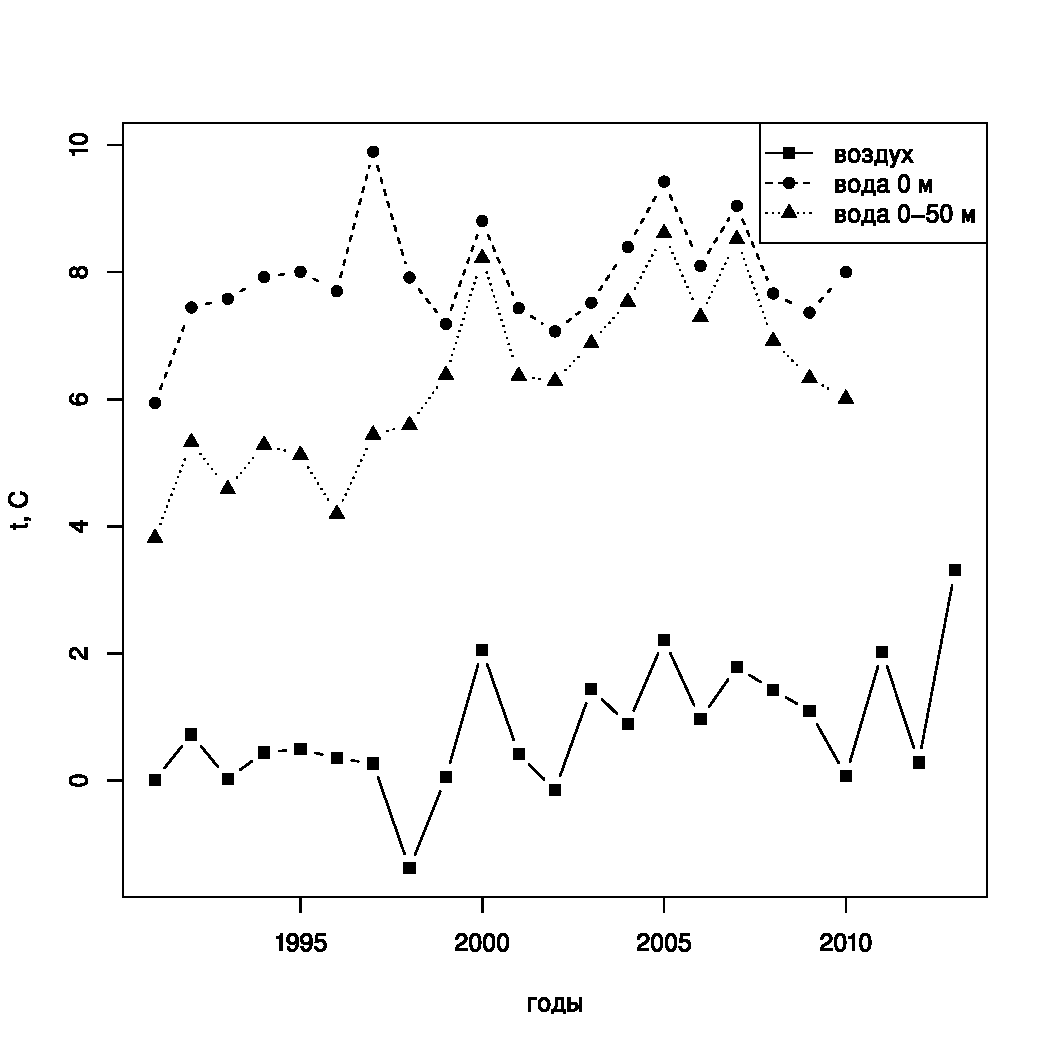
\includegraphics[width=\textwidth]{../temperatures_water_air/White_temp_air_water_dynamic1.pdf}
    \caption{Динамика среднегодовых температур воды и воздуха в Кандалакшском заливе Белого моря}
    \label{ris:White_temp_year_dynamic}
	\end{figure}

Среднегодовая температура воздуха и температура воды достоверно скоррелированы (корреляция Спирмена для температуры поверхности воды: $\rho = 0,3, p = 0,0035$, для температуры верхнего 50-метрового слоя: $\rho = 0,7, p = 0,0008$).

Использование среднегодовых значений температуры скрывает сезонное варьирование, которое может быть принципиально важно для поселений маком (например: \cite{Beukema_et_al_1998, Beukema_Dekker_2003, Beukema_et_al_2009}). 
Корреляция среднесезонных температур воздуха и поверхности воды выше, чем среднегодовых значений (корреляция Спирмена для температуры поверхности воды: $\rho = 0,92, p < 0,0001$ (рис.~\ref{ris:White_temp_water_vs_air_seasons}). 
	\begin{figure}[p]
    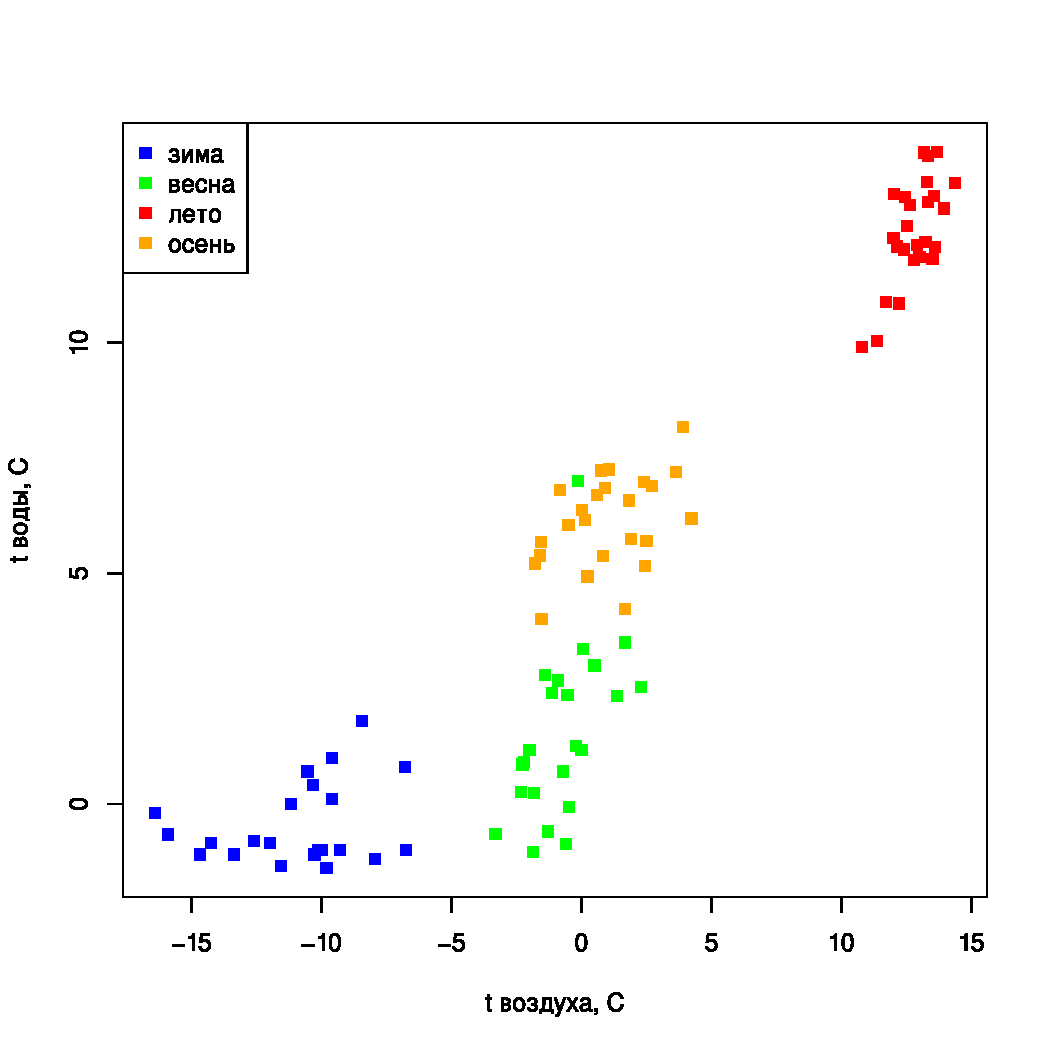
\includegraphics[width=\textwidth]{../temperatures_water_air/temp_air_water1.pdf}
    \caption{Соответсвие среднесезонных температур воды и воздуха в Кандалакшском заливе Белого моря}
    \label{ris:White_temp_water_vs_air_seasons}
	\end{figure}
Динамика средней температуры воды в разные сезоны представлена на рисунке~\ref{ris:White_temp_seasons_dynamic}.
	\begin{figure}[p]
    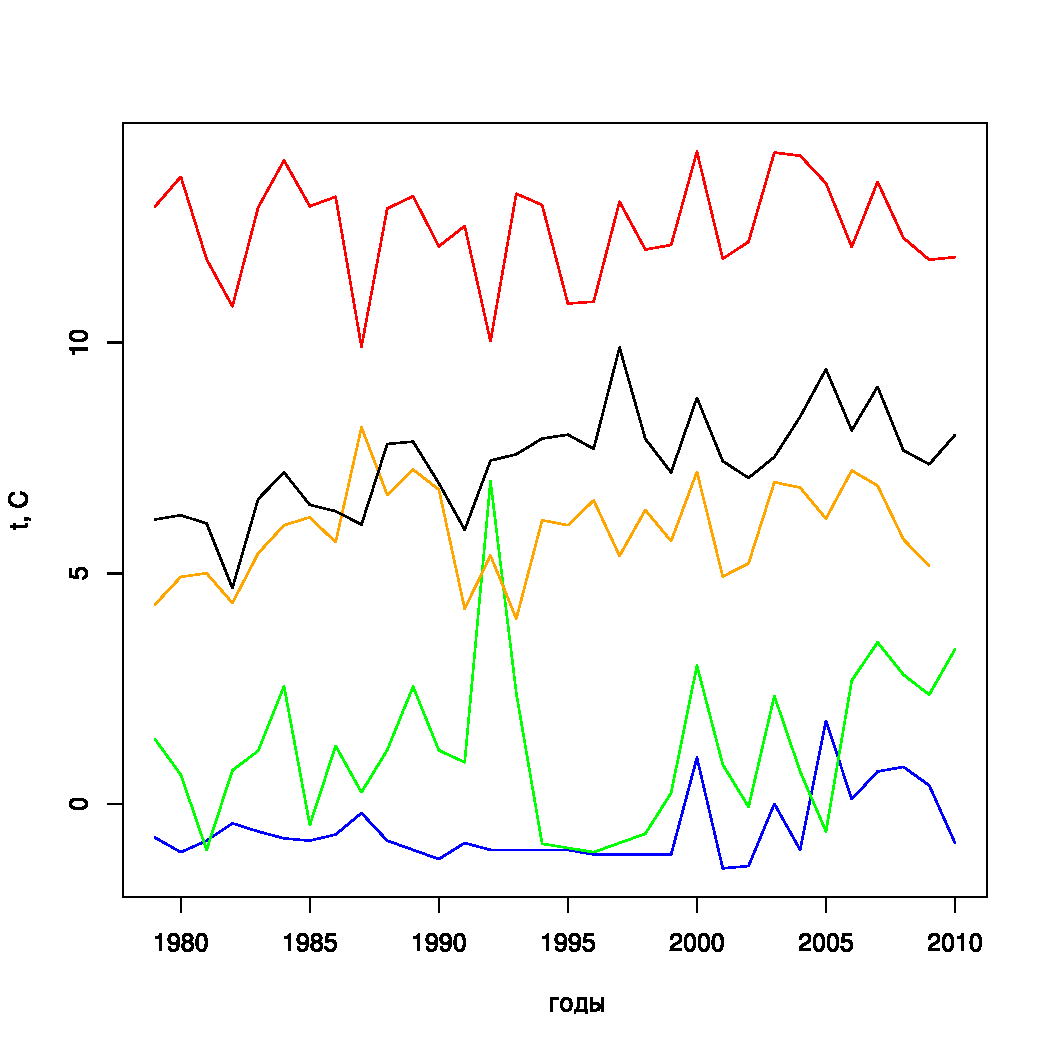
\includegraphics[width=\textwidth]{../White_Sea/temperature_Kartesh/t_mean_season_year1.pdf}
    \caption{Динамика среднесезонной температуры воды в губе Чупа(Кандалакшский залив Белого моря) (\cite{Berger_et_al_2003})}

{\footnotesize Примечание: t, C~--- температура поверхности воды: синий~--- зимняя, зеленый~--- веснняя, красный~--- летняя, оранжевый~--- осенняя, черный~--- среднегодовая. }
    \label{ris:White_temp_seasons_dynamic}
	\end{figure}


Таким образом, динамика среднегодовых температур в Белом море характеризуется значительными флуктуациями.
При рассмотрении сезонных данных оказывается, что средневесенняя температура наиболее вариабельна, в то время как среднезимняя до $1999$ года была относительно стабильна, а в дальнейшем также значительно варьировала из года в год (рис.~\ref{ris:White_temp_seasons_dynamic}).

		\subsection{Баренцево море}
Для Баренцева моря были использованы данные по динамике температур на разрезе Кольский меридиан (\cite{pinro}). 
Наиболее адекватными данными для оценки динамики литоральных температурных условий представляются данные о средней температуре в верхнем 50-метровом слое воды на прибрежных станциях (рис.~\ref{ris:Barents_temp_dynamic}).
	\begin{figure}[p]
    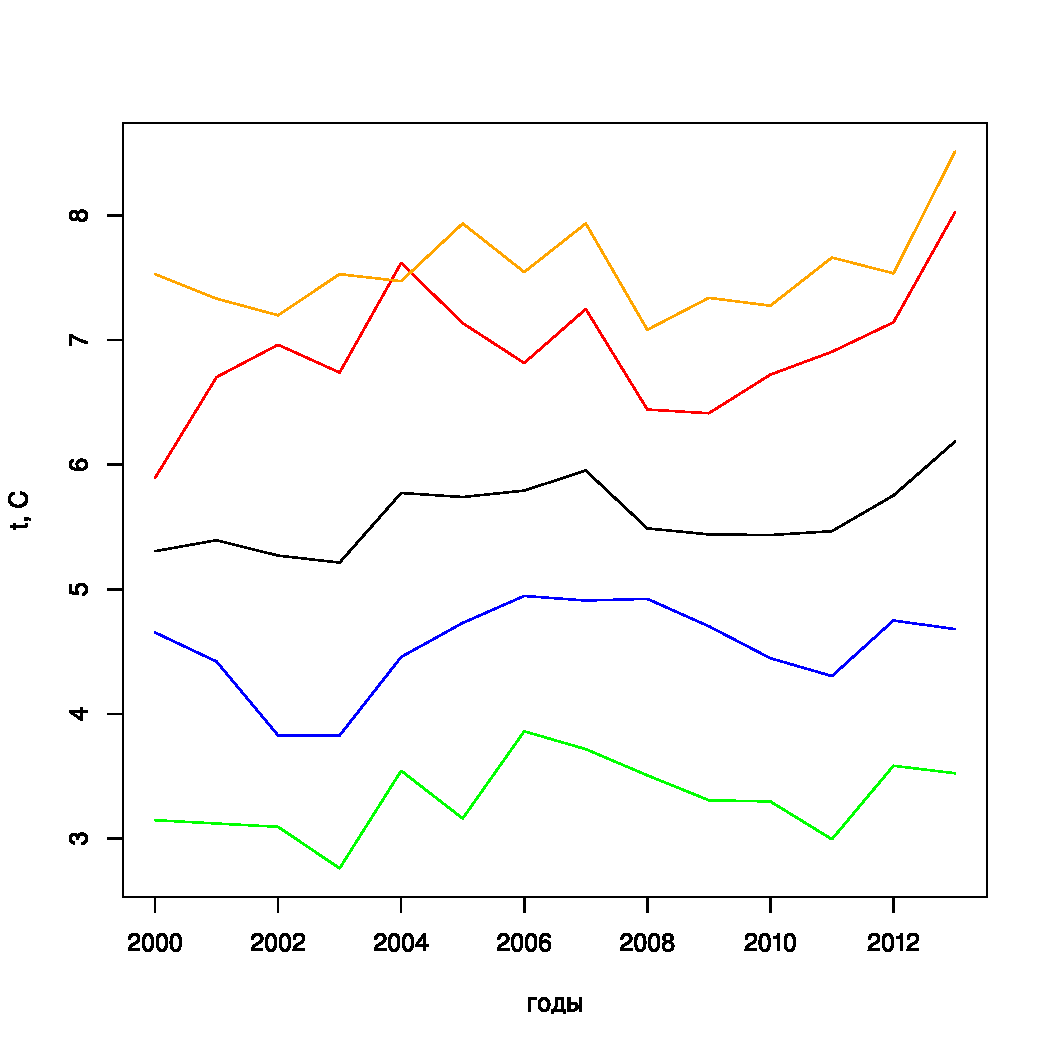
\includegraphics[width=\textwidth]{../Barenc_Sea/temperature/t_air_mean_season_year1.pdf}
    \caption{Динамика температуры воды верхнего 50-метрового слоя на разрезе Кольский меридиан(станции 1-3) (\cite{pinro})}

{\footnotesize Примечание: t, C~--- температура поверхности воды: синий~--- зимняя, зеленый~--- веснняя, красный~--- летняя, оранжевый~--- осенняя, черный~--- среднегодовая. }
    \label{ris:Barents_temp_dynamic}
	\end{figure}

В Баренцевом море за иследованное время ($2002 - 2008$) можно говорить об относительно более теплом периоде~--- с $2004$ по $2007$ год.
При этом данное потепление охватывало все сезоны (рис.~\ref{ris:Barents_temp_dynamic}).
Если рассматривать среднезимние температуры, то относительно теплый период захватывает также $2008$ год.


\bigskip

Таким образом, условия обитания маком в Белом и Баренцевом море различаются по многим параметрам.
Температурный режим прибрежной части Кандалакшского залива Белого характеризует более значительные сезонные колебания(рис.~\ref{ris:temp_White_Barents}).
	\begin{figure}[p]
    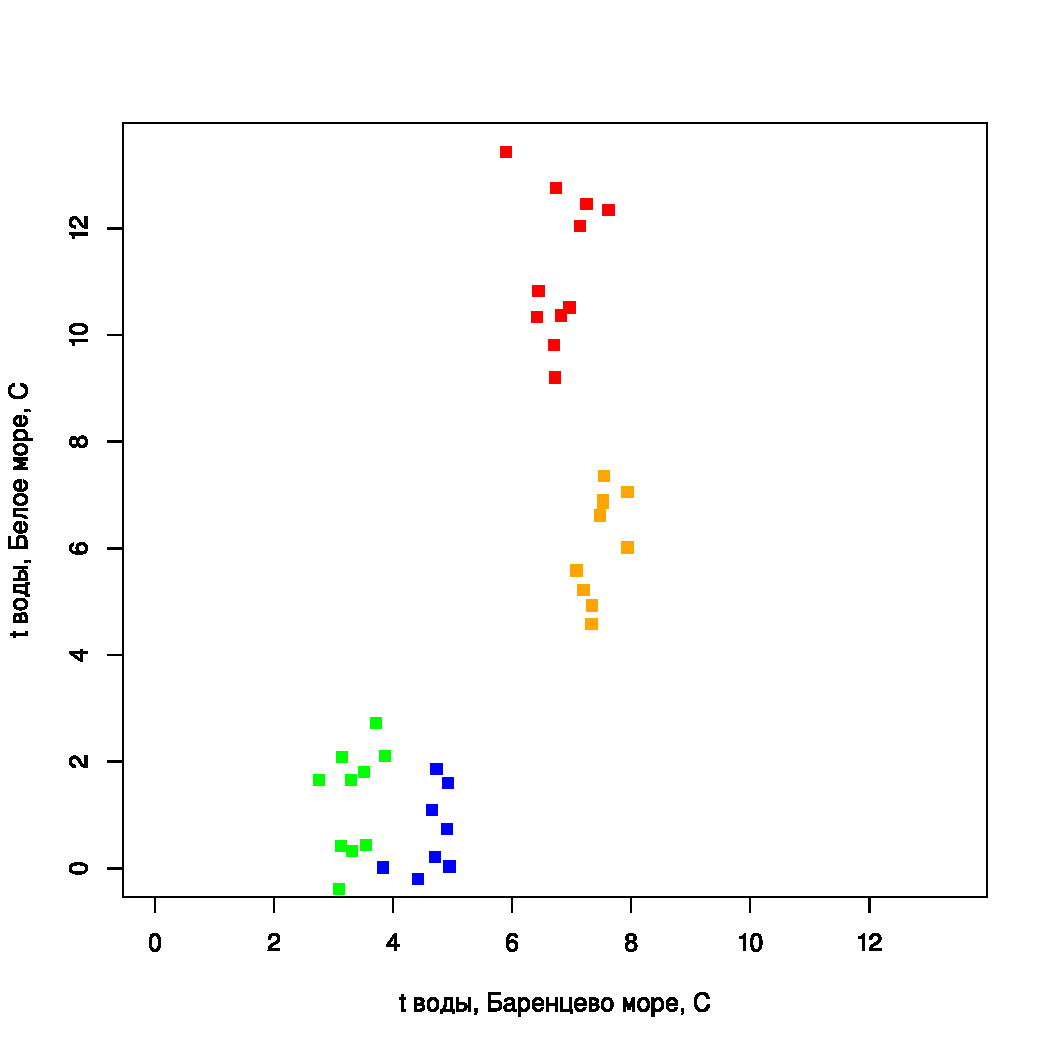
\includegraphics[width=\textwidth]{../temperatures_water_air/temp_White_Barents1.pdf}
    \caption{Соотношение среднесезонных температур в верхнем 50-метровом слоях воды в Белом и Баренцевом морях}

{\footnotesize Примечание: t, C~--- температура поверхности воды: синий~--- зимняя, зеленый~--- веснняя, красный~--- летняя, оранжевый~--- осенняя}
    \label{ris:temp_White_Barents}
	\end{figure}
В пределах каждого сезона межгодовые изменения в Белом море также выше, чем в Баренцевом.
Кроме того, различается сезонность хода температур. 
В Белом море лето является наиболее теплым сезоном, а зима~--- наиболее холодным.
Для Баренцева моря гидрологическая сезонность сдвинута относительно календарной: самый теплый сезон это осень, а самый холодный~--- весна.

\afterpage{\clearpage}
